\documentclass[border=10pt]{standalone}
\usepackage{pgfplots}
\pgfplotsset{compat=1.18}
\begin{document}
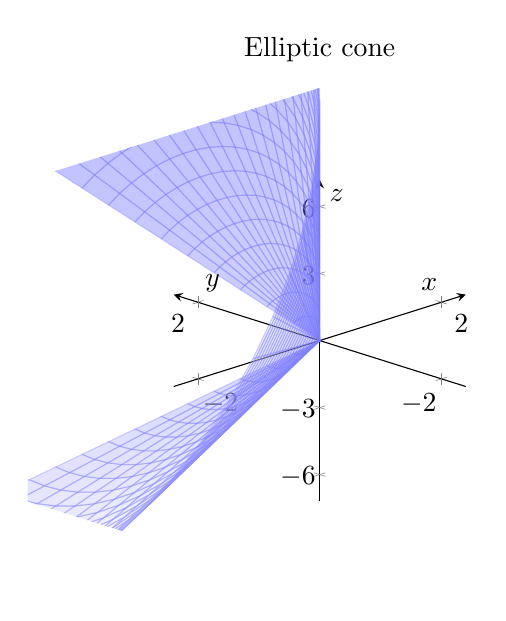
\begin{tikzpicture}
\begin{axis}[
  width=9cm,
  height=8cm,
  axis lines=center,
  xlabel=$x$, ylabel=$y$, zlabel=$z$,
  xmin=-2.4, xmax=2.4,
  ymin=-2.4, ymax=2.4,
  zmin=-7.2, zmax=7.2,
  view={-45}{22},
  title={Elliptic cone},
  samples=45,
  samples y=24,
  domain=-2.2:2.2,
  y domain=0:2*pi,
  grid=major,
  ztick={-6,-3,0,3,6},
]
\addplot3[
  surf,
  shader=flat,
  opacity=0.35,
  colormap={bluewhite}{color=(white) color=(blue)},
  draw=blue!50,
  domain=-2.2:2.2,
  y domain=0:2*pi,
  variable=t,
  variable y=u,
] ({u*cos(deg(t))}, {u}, {3*u*sin(deg(t))});
\end{axis}
\end{tikzpicture}
\end{document}
